\documentclass[a4paper,10pt]{scrartcl}

%Basic 
\usepackage[utf8]{inputenc}
\usepackage[ngerman]{babel}
\usepackage[T1]{fontenc}

%Titel Seite
\title{CLOUD INFRASTRUCTURE}
\subtitle{Lab-xx}
\author{Giorgio Vincenti, Samuel Krieg}
\date{\today}


%Kopf, Fusszeile
\usepackage{fancyhdr}
\pagestyle{fancy}
\lhead{ \begin{picture}(0,0) \put(0,0){
\includegraphics[width=3cm]{./pictures/hsrlogo.png}} \end{picture}}
\chead{}
\rhead{Seite \thepage}
\lfoot{Cloud Infrastructure \\Lab-xx}
\cfoot{Giorgio Vincenti und Samuel Krieg}
\rfoot{\today}
\renewcommand{\headrulewidth}{0.4pt}

%Bilder
\usepackage{graphicx}

%Tabellen
\usepackage{booktabs}

\begin{document}

\maketitle
\tableofcontents
\newpage

\section{Section}
Text

\subsection{Subsection}
Text

\subsubsection{Subsubsection}
Text

\section{Bilder}
\begin{figure} [h]
\begin{center}
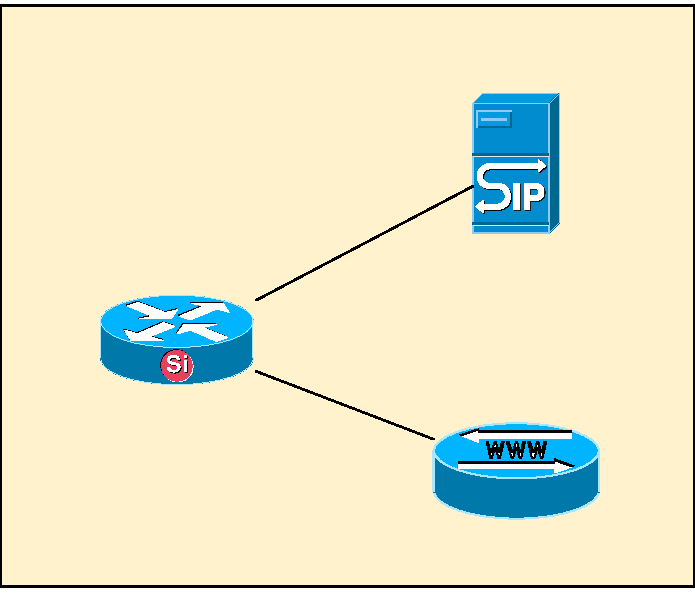
\includegraphics[width=0.50\textwidth]{./pictures/sample_picture.pdf}
\caption{Bild Unterschrift}
\label{Bild Referenz}
\end{center}
\end{figure}

\section{Tabellen}
\begin{center}
    \begin{tabular}{@{} l l r@{}}\toprule    
    {Stockwerk} & {Hostname} & {Anzahl Ports}\\ \midrule
    1 & DataCSW01 & 12\\ \addlinespace
    & DataCSW03 & 12\\ \addlinespace
    & DataCSW04 & 12\\ \addlinespace
    2& DataCSW02 & 24\\
    \bottomrule
    \end{tabular}
\end{center}


\end{document}
